% Resultate
\section{Resultate}

\subsection{Bekannte Fehler}

\subsubsection{iOS - Add to homescreen}
Eine sehr nützliche Funktionalität, welche Apple im Mobile Safari-Browser anbietet ist die \emph{Add to homescreen}-Funktion.

\begin{figure}[H]
\subfigure{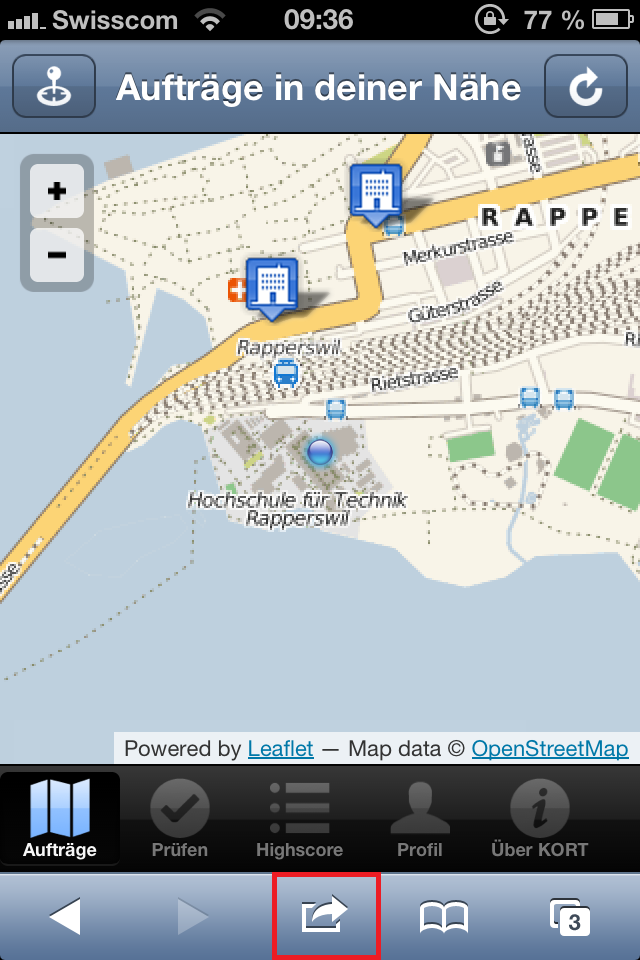
\includegraphics[width=0.23\textwidth]{images/bugs/kort-add_to_homescreen_1}}
\hfill
\subfigure{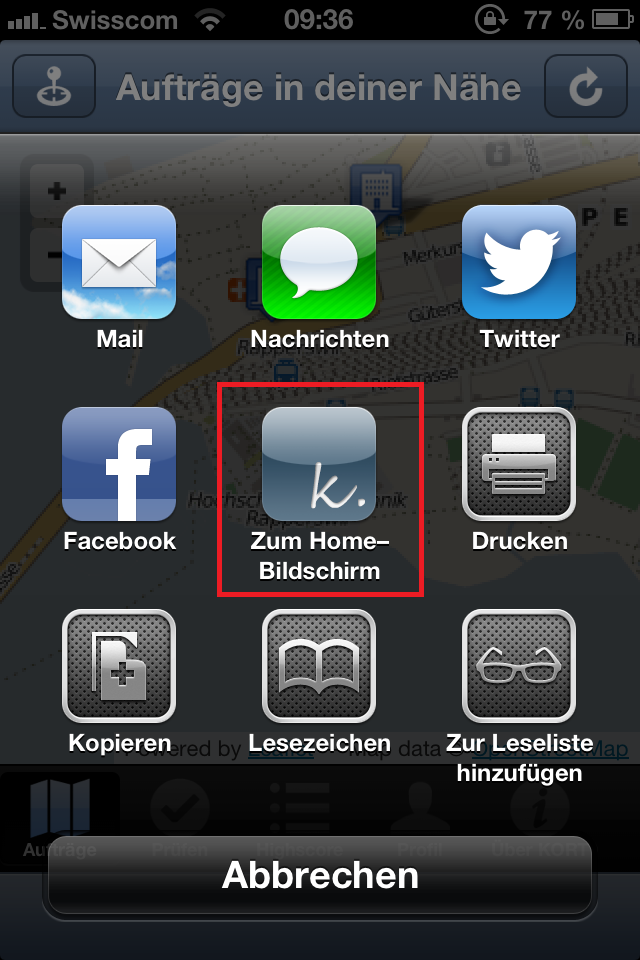
\includegraphics[width=0.23\textwidth]{images/bugs/kort-add_to_homescreen_2}}
\hfill
\subfigure{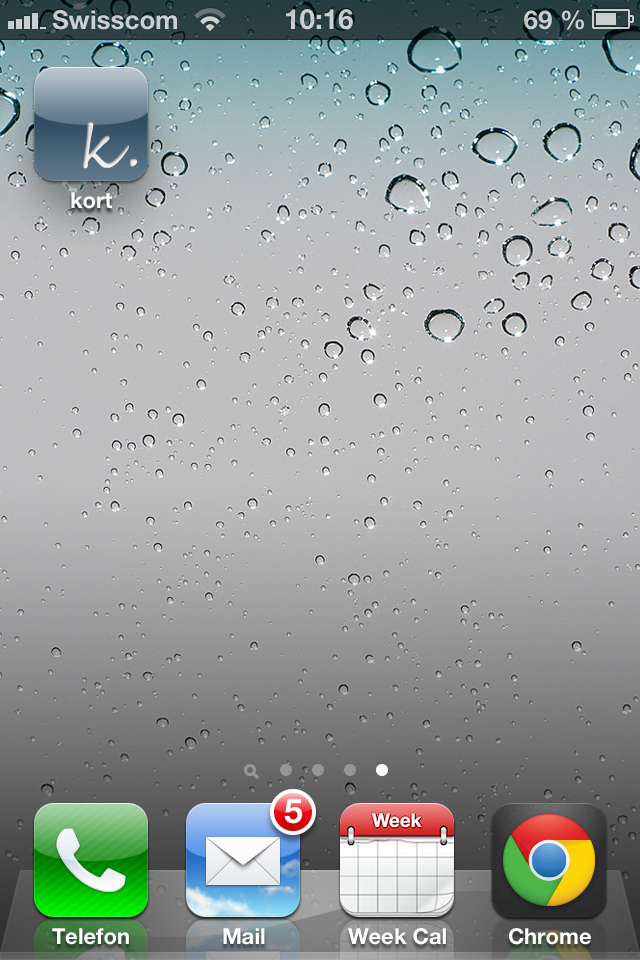
\includegraphics[width=0.23\textwidth]{images/bugs/kort-add_to_homescreen_3}}
\hfill
\subfigure{
\includegraphics[width=0.23\textwidth]{images/bugs/kort-add_to_homescreen_4}}
\caption{iOS - "`Add to homescreen"'-Funktion}
\end{figure}

Dadurch wird ein App-ähnlicher Bookmark der aktuellen Webseite auf dem Homescreen erstellt.
Dieser erhält ein hinterlegtes Icon und einen Titel.
Beim Starten der App erscheint ein Splashscreen, welchen man ebenfalls in der Webseite definieren kann. Zudem öffnet sich der Browser ohne jegliche Toolbars wie der Adressleiste oder der Navigationsbar.

Leider hat die verwendete Version (2.1.0) des Sencha Touch Frameworks Fehler bei der Anzeige von einigen GUI-Komponenten.
So werden in unserem Fall die Karte (Aufträge) und alle Listen (Prüfen, Highscore) nicht korrekt dargestellt.

\subsubsection{App Build}
Wie in Abschnitt \ref{sencha-cmd} beschrieben, basiert die App vollständig auf dem Sencha-eigenen Build-Tool \emph{Sencha Cmd 3.0.0}. Darin sind aber noch einige Bugs vorhanden.

Bei \textsc{Kort} besteht dabei ein Problem bei der fest eingebauten Komprimierung der JavaScript-Sourcen.
Während diesem Prozess werden lokale Variablennamen mit einzelnen Buchstaben abgekürzt.
Dabei treten Konflikte mit der Leaflet-Library auf, welche den Buchstaben \emph{L} als Namespace verwendet.